% =====================================================================
%  CSC_43M04_EP — Computer Vision with Deep Learning (École Polytechnique)
%  Team 8 — Florian Guillaumey & Andrea Signoretti
%  Report (merged): unified two-track report (Closed World + Open World),
%  Track~A section refreshed with the ResNet50 backbone and ablation results.
%
%  CVPR double-column template. Requires cvpr.sty + ieeenat_fullname.bst
%  (already in docs/). silence.sty and cleveref.sty stubs are provided for
%  TeX installs that lack them.
%
%  Build (from docs/report_merged/):
%    export TEXINPUTS="$PWD:" BSTINPUTS="$PWD:" BIBINPUTS="$PWD:"
%    pdflatex report && bibtex report && pdflatex report && pdflatex report
%
%  Figures live in figures/ and are gathered at the END after \clearpage.
% =====================================================================
\documentclass[10pt,twocolumn,letterpaper]{article}

\usepackage{cvpr}              % final (camera-ready) mode
\usepackage{graphicx}
\usepackage{amsmath,amssymb}
\usepackage{booktabs}
\usepackage{xcolor}
\usepackage[pagebackref,breaklinks,colorlinks,allcolors=blue]{hyperref}

\graphicspath{{figures/}}

% Reduce margins to gain ~2 extra lines per page
\addtolength{\textheight}{2.0cm}
\addtolength{\topmargin}{-1.0cm}
\addtolength{\textwidth}{0.6cm}
\addtolength{\oddsidemargin}{-0.3cm}
\addtolength{\evensidemargin}{-0.3cm}

% Make all section headings bold
\makeatletter
\renewcommand\section{\@startsection{section}{1}{\z@}%
  {-3.5ex \@plus -1ex \@minus -.2ex}%
  {2.3ex \@plus.2ex}%
  {\normalfont\Large\bfseries}}
\renewcommand\subsection{\@startsection{subsection}{2}{\z@}%
  {-3.25ex\@plus -1ex \@minus -.2ex}%
  {1.5ex \@plus .2ex}%
  {\normalfont\large\bfseries}}
\renewcommand\subsubsection{\@startsection{subsubsection}{3}{\z@}%
  {-3.25ex\@plus -1ex \@minus -.2ex}%
  {1.5ex \@plus .2ex}%
  {\normalfont\normalsize\bfseries}}
\renewcommand\paragraph{\@startsection{paragraph}{4}{\z@}%
  {1.5ex \@plus .5ex \@minus .2ex}%
  {-1em}%
  {\normalfont\normalsize\bfseries}}
\makeatother
% \textbb{} is now just a passthrough — all section headings are already bold
\providecommand{\textbb}[1]{#1}

\def\cvprPaperID{8}
\def\confName{CSC\_43M04\_EP — Modal d'informatique}
\def\confYear{2026}

\title{%
  \textbf{What Happens Next?}\\[0.15em]
  \textbf{Video Action Prediction on Something-Something\,V2}}

\author{%
  Andrea \textsc{Signoretti}
  \quad
  Florian \textsc{Guillaumey}\\[0.3em]
  \small{\'Ecole Polytechnique --- CSC\_43M04\_EP --- 8 June 2026}\\
  \scriptsize{\texttt{andrea.signoretti@polytechnique.edu}\quad
  \texttt{florian.guillaumey@polytechnique.edu}
  }\\
  \scriptsize{\url{https://github.com/Fl0972/What-Happens-Next-Video-Action-Prediction-on-Something-Something-V2}}
}

\begin{document}
\maketitle
\thispagestyle{plain}
\pagestyle{plain}
\vspace{-1.0em}

% =====================================================================
\begin{abstract}
We present in this report a two-track study of temporal action prediction on a 33-class subset
of Something-Something\,V2 (SSv2)~\cite{goyal2017ssv2}, ``What Happens Next?'':
only the first ${\approx}40\%$ of each clip (four JPEG frames) is given, so the
outcome is withheld and classification must reason about motion. In
\textbf{Track~A (Closed World)}, where pretraining is forbidden, our study shows that
\emph{where} a model mixes time matters more than \emph{how much} capacity it
has: Temporal-Shift-Module~\cite{lin2019tsm} (TSM), which mixes frames
\emph{before} spatial pooling, beats VideoFormer-Lite (VFL, global
post-pooling attention) by $+3.0$\,pp at matched backbone size, and scaling
its backbone from ResNet18 to ResNet50 then adds a further $+3.4$\,pp to reach
\textbf{42.85\%} \texttt{val\_dir} (our best single model). A five-model
log-softmax ensemble of TSM and VFL variants with test-time augmentation is our best submission and 
reaches \textbf{0.4785} public / \textbf{0.4547} private Kaggle top-1 score (16th). In
\textbf{Track~B (Open World)}, we fine-tune V-JEPA\,2~\cite{bardes2025vjepa2}
and VideoMAE~\cite{tong2022videomae} backbones with progressive unfreezing,
layer-wise learning-rate decay, window-capped source-frame re-extraction and
pseudo-labelling, then build a 14-model uniform ensemble reaching
\textbf{0.6586} Kaggle top-1 (16th also). We document a
self-discovered data-leakage event (a discarded 0.81 submission) and show that
ensemble diversity across architecture families beats single-family or
learned-weight ensembling. Failure analysis attributes the residual errors to
real-vs-pretended and direction-ambiguous classes that four frames
under-determine.
\end{abstract}

% =====================================================================
\section{Problem Description}
\label{sec:problem}

\paragraph{Task.}
The challenge classifies four-frame JPEG clips into one of 33 motion-defined
action classes (e.g.\ \emph{Pouring something into something}, \emph{Pulling
something from left to right}). Crucially, each clip contains only the
\emph{anticipatory} portion of the source SSv2 video---the shipped
\texttt{frame\_003} sits at a median fraction of $0.40$ of the source clip---so
the action's outcome is deliberately withheld and the task probes motion
prediction, not final-state recognition~\cite{goyal2017ssv2}.

\paragraph{Dataset.}
The split provides $44{,}993$ training clips, $6{,}745$ validation clips and
$6{,}913$ test clips over 33 classes (numeric prefixes 000--032; class~027 is
absent from training). Classes are heavily imbalanced: the largest (009,
\emph{Moving something up}) has $3{,}170$ examples while the smallest (026,
\emph{Spilling something next to something}) has only 162, a ratio of
$19.6\times$. The KL divergence between training and validation class
distributions is $0.088$, confirming the splits are representative.

\paragraph{\textbf{Evaluation and tracks.}}
Submissions are scored by top-1 accuracy on a public+private Kaggle leaderboard
over two stages (Stage~1, intermediate; Stage~2, final); top-5 is tracked
internally. The provided baseline reaches ${\approx}0.55$ private and the
second-place public reference is $0.74$; our final submissions placed
\textbf{16th in both tracks} (counting the multiple accounts fielded by some
teams). Following the challenge, we report two regimes. \textbf{Track~A (Closed
World)} prohibits pretrained models and external data---all spatial features,
temporal dynamics and class boundaries are learned from scratch on the four
provided frames. \textbf{Track~B (Open World)} permits pretrained backbones and
external corpora but not future frames or test labels. The task is hard for
three reasons: (i)~labels are motion-defined, defeating appearance-only
models~\cite{goyal2017ssv2}; (ii)~four frames is an order of magnitude below the
8--32 standard in video recognition~\cite{lin2019tsm,bertasius2021timesformer};
(iii)~the discriminative cue---the action's outcome---is withheld by
construction.

% =====================================================================
\section{Methods}
\label{sec:method}

\subsection{Track A --- Closed World}
\label{sec:trackA}
The pipeline evolved through several iterations on an internal training-split,
all trained from scratch (the closed track forbids pretraining and external
data). Our guiding hypothesis is that, without pretraining, \emph{every
parameter spent on temporal modelling is one not spent learning spatial
features}, favouring parameter-free temporal mechanisms over heavy temporal
heads --- and that \emph{where} in the network temporal information is mixed
matters as much as how it is mixed.

\subsubsection{Architecture family and complexity}
\label{sec:arch}
All three Track~A architectures share the contract $(B, T, C, H, W) \to
(B, 33)$ with $T{=}4$, $H{=}W{=}224$, and a ResNet
backbone~\cite{he2016resnet} mapping each frame to a $512$-d (R18) or
$2048$-d (R50) vector after global average pooling (Fig.~\ref{fig:arch}). \textbf{CNNBaseline} and
\textbf{CNN-LSTM} simply average (resp.\ recurrently combine) the $T$ pooled
features --- weak baselines ($\approx\!11.2$\,M params) since BPTT on
four-step sequences barely helps. The two strong families differ in
\emph{where} they mix time relative to spatial pooling.

\noindent\textbf{TSM-ResNet}~\cite{lin2019tsm} re-indexes, \emph{inside every
residual block and before every convolution}, a fraction
$1/\text{fold\_div}$ of channels one step backward and another
$1/\text{fold\_div}$ one step forward in time:
\begin{equation}
  \text{TSM}(\mathbf{x})_{t,c} = \begin{cases}
  \mathbf{x}_{t-1,c} & c < C/4 \\
  \mathbf{x}_{t+1,c} & C/4 \leq c < C/2 \\
  \mathbf{x}_{t,c}   & \text{otherwise,}
  \end{cases}
  \label{eq:tsm}
\end{equation}
at \emph{zero} parameter cost, while spatial resolution is still full. The $T$
final per-frame vectors are averaged and a linear head $d\!\times\!33$ yields
the logits, so the total cost is exactly backbone $+$ head:
$\approx\!11.2$\,M (R18) and $\approx\!23.6$\,M (R50, $23.5$\,M of which is the
backbone). TSM was designed for SSv2-style motion labels and is a strong prior
here (Fig.~\ref{fig:arch}).

\noindent\textbf{VideoFormer-Lite (VFL)} is our own design --- a
from-scratch-budget distillation of ViT~\cite{dosovitskiy2021vit} and
TimeSformer~\cite{bertasius2021timesformer} ideas that treats whole
\emph{frames}, not space-time patches, as tokens. A ResNet18 encodes each
frame \emph{independently} into a vector of size $d{=}512$, a learnable
\texttt{[CLS]} token~\cite{dosovitskiy2021vit} is appended ($T{+}1{=}5$
tokens), and $n_\ell$ pre-norm Transformer
blocks~\cite{xiong2020prenorm} (8 heads, ratio $r{=}4$) attend globally over
them \emph{after} pooling has already collapsed each frame to a single
descriptor. Each block costs
\begin{equation}
  P_{\text{block}} = \underbrace{4d^2}_{\text{Q,K,V,O}} +
  \underbrace{2\,r\,d^2}_{\text{MLP}} + \underbrace{4d}_{\text{LN}}
  \approx (4 + 2r)\,d^2 \approx 3.1\text{M},
  \label{eq:vfl_params}
\end{equation}
so $n_\ell{=}3$ adds ${\approx}9.4$\,M to the ${\approx}11.2$\,M backbone, for
${\approx}20.7$\,M total --- nearly twice TSM-ResNet18 for \emph{zero} extra
spatial capacity.

\paragraph{\textbf{Where temporal mixing happens --- the key difference.}}
TSM mixes time at full spatial resolution, before pooling: by block~8, each
frame's representation already encodes a receptive field over all $T$ frames
at the $(h,w)$ level. VFL pools \emph{first} and attends only over $T{+}1$
frame-averaged descriptors --- it never sees motion at the pixel level. On
SSv2, where the cue is typically a single finger or edge moving within a
small region, this matters: TSM keeps the spatial precision the cue lives in;
VFL has already discarded it (Fig.~\ref{fig:arch}). Sec.~\ref{sec:abl}
measures this argument directly.

\subsubsection{Critical frame-count fix}
The single largest gain ($+4.4$\,pp) came from matching \texttt{num\_frames}
to the true clip length (four real frames). $\texttt{num\_frames}{>}4$ forces
\texttt{linspace} interpolation that duplicates frames, so consecutive
identical tokens make Eq.~\eqref{eq:tsm} read the same value twice --- zero
temporal gradient on the shifted channels, corrupting the signal TSM relies
on. Setting $T{=}4$ lifted \texttt{tsm\_ultra\_v2} to $57.73\%$ internal /
$38.25\%$ \texttt{val\_dir} ($+4.41$/$+3.34$\,pp); a first ResNet50 attempt at
the old $T{=}8$ regressed to $45.26\%$ internal (Fig.~\ref{fig:permodel},
Fig.~\ref{fig:backbone}) --- capacity cannot undo corrupted input. Once
$T{=}4$ was enforced, a rotating-fold ResNet50 run reached
\textbf{42.85\%} \texttt{val\_dir}, our best single model: \emph{fix the
pipeline before scaling}.

\subsubsection{Regularisation recipe}
All Track~A models share a regularisation stack (Table~\ref{tab:recipe})
whose critical element is a \emph{warm-up delay}: MixUp~\cite{zhang2018mixup}
and CutMix~\cite{yun2019cutmix} are disabled for the first 10 epochs so the
backbone forms basic per-frame representations before label-mixing starts
--- worth $+36.3$\,pp on VFL alone ($9.45\!\rightarrow\!45.78\%$), since a
randomly-initialised head cannot meaningfully mix labels it cannot yet
distinguish, and early MixUp collapses the representation rather than
regularising it. Two further choices are domain-specific:
\emph{horizontal flip is disabled} (it inverts SSv2's direction-encoded
labels, e.g.\ \emph{Pulling left$\rightarrow$right}), and CutMix probability
is kept low ($p{=}0.25$, a cut patch spans all four frames and often occludes
the defining motion).

\begin{table}[t]
\centering\small
\setlength{\tabcolsep}{4pt}
\begin{tabular}{@{}lll@{}}
\toprule
Technique & Setting & Source \\
\midrule
Reg.\ warm-up      & 10 ep, no MixUp/CutMix & \textbf{this work} \\
MixUp / CutMix     & $\alpha{=}0.2$ / $p{=}0.25$, after\,ep\,10 & \cite{zhang2018mixup,yun2019cutmix} \\
Focal loss         & $\gamma{\in}\{0,1,2\}$ (best $\approx$1) & \cite{lin2017focal} \\
Label smoothing    & $\varepsilon{=}0.1$ & standard \\
RandAugment        & 2 ops, mag.\ 0.5 & standard \\
Random erasing     & $p{=}0.25$ & standard \\
Horizontal flip    & \textbf{disabled} & label semantics \\
Stochastic depth   & DropPath 0.1 & standard \\
Optimiser          & AdamW, lr $10^{-3}$, cosine & standard \\
\bottomrule
\end{tabular}
\caption{Track~A training recipe (best single model: TSM-ResNet50, $T{=}4$,
\texttt{fold\_div}=8, rotating folds, ${\sim}42.85\%$ \texttt{val\_dir}).}
\label{tab:recipe}
\end{table}

\subsubsection{Rotating $k$-fold and ensemble}
\label{sec:rotating}
The strongest checkpoints also have a \emph{rotating-fold} variant retrained on
every fold of the train+val union (held-out fold $=\text{epoch}\bmod k$,
$k{=}5$): higher-bias snapshots contributing uncorrelated errors at inference
(Fig.~\ref{fig:rotating}), worth $+1.2$\,pp for TSM-ResNet18 and $+4.3$\,pp for
VFL (its data-hungry attention head lacks TSM's structural temporal prior and
so benefits more from extra data; Sec.~\ref{sec:abl} shows it saturates at
$k{=}5$).

The final submission fuses \emph{five} checkpoints by log-softmax late fusion
--- averaging in log-probability space down-weights over-confident errors and
rewards agreement among differently-calibrated members: three with 10-crop TTA
(\texttt{tsm\_ultra\_v2}, its rotating-fold variant, and
\texttt{video\_former\_lite\_ultra\_rot}), and two without (\textbf{TSM-ResNet50
rotating}, our best single model at $42.85\%$, and a CE-trained $\gamma{=}0$
TSM variant whose different loss geometry adds complementary calibration). It
reaches \textbf{46.75\%} \texttt{val\_dir} (Fig.~\ref{fig:ensemble}) and
\textbf{0.4785} public / \textbf{0.4547} private on Kaggle --- our best
closed-track score, $+6.2$\,pp over the strongest single model ($0.4163$;
Table~\ref{tab:summary}). TTA alone adds ${\sim}1$\,pp on the strongest single
model (Fig.~\ref{fig:tta}), trading off on direction-encoded classes
(Fig.~\ref{fig:ttatradeoff}) where hflip views push confidences toward the
mirror class even after label-aware remapping.

\subsection{Track B --- Open World}
\label{sec:trackB}
Top SSv2 teams use video transformers pretrained on large unlabelled corpora.
We selected \textbf{VideoMAE}~\cite{tong2022videomae} (masked-autoencoder
pre-training; HuggingFace Kinetics-400 checkpoints) and \textbf{V-JEPA\,2}~\cite{bardes2025vjepa2},
a joint-embedding predictive architecture that reconstructs masked regions in
\emph{feature} space, focusing capacity on semantically relevant motion. We use
the self-supervised \texttt{vjepa2-vitl-fpc64-256} checkpoint, pretrained on
unlabelled video without SSv2 labels---required for integrity
(Sec.~\ref{sec:integrity}).

\paragraph{\textbf{Progressive unfreezing with LLRD.}}
V-JEPA is fine-tuned in three phases with layer-wise LR decay (block $\ell$
gets $\eta\cdot\lambda^{\ell}$, $\lambda{=}0.75$): a frozen attentive probe
reaches $0.672$ EMA internal val, unfreezing the top-6 blocks reaches $0.705$,
and full-encoder fine-tuning reaches $0.728$ internal / $0.6411$
\texttt{val\_dir}. Freezing first stabilises the head and preserves pretrained
feature geometry; the resulting staircase is visible in
Fig.~\ref{fig:vjepacurves}.

\paragraph{\textbf{Window-capped source-frame re-extraction.}}
V-JEPA benefits from 16 frames but only four are shipped; since folder names
encode SSv2 video IDs, the source WebM files are reachable. We match the
shipped \texttt{frame\_003} to source frames by pixel-level MAE to locate the
provided window's end, sample 16 frames within it, and hard-bound the search
to the clip's first 50\% so the withheld outcome ($>60\%$) stays unreachable by
construction (median window fraction $0.39$, max $0.50$; Fig.~\ref{fig:framehist}).

\paragraph{\textbf{Pseudo-labelling.}}
Following noisy-student self-training, the Phase-2 ensemble soft-labelled the
test clips; a $\geq 0.85$ confidence threshold retained \emph{all} 6{,}913
clips (the model is over-confident), so the loop effectively trained on
train\,$\cup$\,test under its own predictions. The resulting V-JEPA-pseudo
reached $0.6519$ \texttt{val\_dir} / $0.6410$ Kaggle, but its widened gap
(Sec.~\ref{sec:results}) signalled over-fitting, so we stopped there.

\paragraph{\textbf{Honest cross-preprocessing ensemble.}}
The final system aggregates 14 checkpoints from three families, each on its
\emph{own} preprocessing (V-JEPA: 6, 16-frame 256\,px window-capped;
VideoMAE-Base/Large K400: 3+3, 4-frame 224\,px; TSM-ResNet50: 2, 4-frame),
combined by \emph{uniform} softmax averaging: diverse, distinct models produce
uncorrelated errors that cancel, so even the weakest member (TSM-ResNet50)
raises the ensemble (Sec.~\ref{sec:results}).

\subsection{Reused vs.\ own code}
\label{sec:reuse}
\emph{Reused:} the course starter repo (Hydra, \texttt{VideoFrameDataset},
\texttt{train.py}); torchvision ResNet~\cite{he2016resnet} and R(2+1)D
backbones; pretrained HuggingFace V-JEPA\,2~\cite{bardes2025vjepa2} and
VideoMAE~\cite{tong2022videomae} checkpoints (Track~B only).
\emph{Our own:} the parameter-free TSM wrapper~\cite{lin2019tsm};
VideoFormer-Lite (Sec.~\ref{sec:arch}); the regularisation-warm-up recipe,
rotating $k$-fold protocol, ablation suite, and log-softmax ensemble/TTA
pipeline; and the full Track~B stack --- window-capped re-extraction,
progressive-unfreezing+LLRD, and noisy-student pseudo-labelling.

% =====================================================================
\section{Results}
\label{sec:results}

\paragraph{\textbf{Overall.}}
Table~\ref{tab:summary} reports headline results with Kaggle scores for
\emph{both} tracks. Track~A reaches \textbf{46.75\%} \texttt{val\_dir} /
\textbf{0.4785} Kaggle public from scratch; Track~B reaches \textbf{0.6586}
Kaggle top-1 ($65.19\%$ internal val) with the 14-model uniform ensemble ---
above the $0.55$ baseline and close to the $0.74$ second-place reference. The
${\approx}18$-pp Kaggle gap between the tracks' best submissions closely tracks
the ${\sim}18$-pp \texttt{val\_dir} gap: forgoing large-scale self-supervised
pretraining costs about the same whether measured internally or on the
independent Kaggle distribution --- both tracks generalise with a comparable,
small, positive offset (calibration below).

\begin{table}[t]
\centering\footnotesize
\setlength{\tabcolsep}{2.5pt}
\begin{tabular}{@{}clccc@{}}
\toprule
Trk & Method & \texttt{val\_dir} & Kgl\,pub. & Kgl\,priv. \\
\midrule
A & TSM-R18 (single, +TTA) & 41.68\% & 0.4163 & 0.3881 \\
A & TSM-R18 (single)       & 38.25\% & 0.3576 & 0.3442 \\
A & VFL-Ultra (single)     & 32.11\% & ---    & --- \\
A & TSM-R50 rot.\ (single) & \textbf{42.85}\% & --- & --- \\
A & 3-model ens.\ +TTA     & 44.03\% & 0.4508 & 0.4260 \\
A & \textbf{5-model ens.}\ (R50) & \textbf{46.75}\% & \textbf{0.4785} & \textbf{0.4547} \\
\midrule
B & V-JEPA-ft standalone   & 64.11\% & \multicolumn{2}{c}{0.6361} \\
B & V-JEPA-pseudo          & 65.19\% & \multicolumn{2}{c}{0.6410} \\
B & \textbf{14-uniform}    & \textbf{65.19\%} & \multicolumn{2}{c}{\textbf{0.6586}} \\
\bottomrule
\end{tabular}
\caption{Summary of Track~A and Track~B results (\texttt{val\_dir} = internal
top-1; Kgl = Kaggle public/private top-1, reported separately for Track~A
where the gap is informative, combined for Track~B). Track~A ResNet50 has no
solo Kaggle submission --- evaluated as an ensemble member only.}
\label{tab:summary}
\end{table}

\subsection{Track~A ablations}
\label{sec:abl}
\paragraph{\textbf{Regularisation warm-up ($+36.3$\,pp).}}
Single variable: without warm-up VFL stalls at $9.45\%$ (killed at epoch 4)
and R(2+1)D at $10.78\%$; with a 10-epoch warm-up VFL reaches $45.78\%$.
The effect transfers across architectures: a general property of cold-start
training with label-mixing, not an architecture-specific quirk.

\paragraph{\textbf{Frame count ($+4.4$\,pp).}}
$T{=}5\!\rightarrow\!4$ improves internal val by $+4.41$\,pp
($53.32\!\rightarrow\!57.73$) and \texttt{val\_dir} by $+3.34$\,pp
($34.91\!\rightarrow\!38.25$); the \emph{first} ResNet50 attempt at the
old $T{=}8$ regressed ${\approx}12$\,pp below the $T{=}4$ ResNet18 internal score
(Fig.~\ref{fig:permodel}).

\paragraph{\textbf{Architecture: TSM vs.\ VFL ($+3.0$\,pp for local mixing).}}
At matched settings (rotating folds, $T{=}4$, ResNet18, no TTA), TSM reaches
$39.45\%$ \texttt{val\_dir} vs.\ VFL's $36.44\%$ ($+3.01$\,pp). With all else
fixed, the only difference is \emph{where} the two mix time --- before pooling
(TSM) or after (VFL) --- so this is the controlled test of
Sec.~\ref{sec:arch}'s argument, and local mixing wins clearly, as expected for
labels defined by small, spatially-localised motion cues that pooling destroys.

\paragraph{\textbf{Backbone scale-up, done right ($+3.4$\,pp).}}
With $T{=}4$ and rotating folds fixed, swapping ResNet18 for ResNet50
($11.2\!\rightarrow\!23.6$\,M params) brings
$39.45\%\!\rightarrow\!42.85\%$ \texttt{val\_dir} ($+3.40$\,pp,
Fig.~\ref{fig:backbone}). Together with the $T{=}8$ regression above, this
closes the loop on our central claim: \emph{capacity is useless on top of a
corrupted temporal signal, but pays off once the signal is correct} --- the
same $2.1\times$ parameter increase that wasted itself on duplicated frames at
$T{=}8$ converts cleanly into accuracy at $T{=}4$.

\paragraph{\textbf{Focal-loss $\gamma$ sweep and VFL ablations (small, informative effects).}}
With TSM-ResNet18 otherwise frozen, CE ($\gamma{=}0$) reaches $38.92\%$,
$\gamma{=}1$ reaches $39.50\%$, $\gamma{=}2$ reaches $39.45\%$
(Fig.~\ref{fig:abla_tsm}): any focal weighting beats CE by
${\approx}0.5$\,pp, but $\gamma{\in}[1,2]$ is within noise --- the gain comes
from \emph{having} a confusable-pair-aware loss, not tuning it finely. The CE
model still adds $+0.52$\,pp to the final ensemble (Sec.~\ref{sec:rotating}): a
different loss geometry gives a different calibration, exactly what log-softmax
fusion exploits. On VFL (Fig.~\ref{fig:abla_vfl}), dropping from 3 to 2
Transformer layers (Eq.~\eqref{eq:vfl_params}: $-3.1$\,M) costs $-1.08$\,pp
($36.44\!\rightarrow\!35.36\%$), and over-rotating from 5 to 10 folds costs a
further $-0.46$\,pp --- VFL saturates its data-utilisation capacity at $k{=}5$,
so extra coverage just adds gradient noise from smaller validation folds.

\paragraph{\textbf{Ensemble components and leave-one-out.}}
\label{sec:loo}
Table~\ref{tab:loo} (Fig.~\ref{fig:loo}) leaves out one member at a time from
the final 5-model ensemble (46.75\%). Every member is necessary, but the
\emph{margins} are revealing: dropping the ResNet50 model costs $-1.33$\,pp,
far the largest drop --- more than any same-backbone TSM-ResNet18 variant
($-0.31$ to $-0.47$\,pp) or the architecturally distinct VFL ($-0.64$\,pp).
\textbf{Backbone diversity contributes more than architecture-family diversity
at matched capacity}: TSM and VFL stay complementary, but the largest source of
useful, decorrelated error is a model that simply \emph{sees more} (deeper
backbone), not one that sees \emph{differently}.

\begin{table}[t]
\centering\small
\begin{tabular}{@{}lcc@{}}
\toprule
Configuration & Top-1 & $\Delta$ \\
\midrule
Full ensemble (5 models)             & \textbf{46.75\%} & --- \\
\;$-$ TSM-ResNet50 (rot)             & 45.41\% & $-1.33$ \\
\;$-$ VFL-Ultra-rot $+$TTA           & 46.11\% & $-0.64$ \\
\;$-$ TSM-no-focal (rot)             & 46.23\% & $-0.52$ \\
\;$-$ TSM-Ultra-v2-rot $+$TTA        & 46.27\% & $-0.47$ \\
\;$-$ TSM-Ultra-v2 $+$TTA            & 46.43\% & $-0.31$ \\
\bottomrule
\end{tabular}
\caption{Track~A leave-one-out on \texttt{val\_dir} for the final 5-model
ensemble (46.75\%). Every component is necessary; the ResNet50 backbone is by
far the dominant contributor, ahead of the architecturally distinct VFL.}
\label{tab:loo}
\end{table}

\subsection{Track~B ablations}
\paragraph{\textbf{Honest Kaggle progression.}}
Table~\ref{tab:kaggle} (Fig.~\ref{fig:kagglejourney}) traces the key honest
milestones. The $21$\,pp gap between the discarded leaky run ($0.81$) and the
first honest baseline ($0.6361$) quantifies what data leakage was buying; every
later point came from legitimate architectural diversity. Fig.~\ref{fig:enssize}
plots Kaggle vs.\ ensemble size: returns stay positive at $n{=}14$, and the
$6$-model V-JEPA-only mix underperforms the $9$-model uniform mix despite
higher individual accuracies --- a first hint that family diversity matters
more than per-model strength.

\begin{table}[t]
\centering\small
\setlength{\tabcolsep}{5pt}
\begin{tabular}{@{}lcc@{}}
\toprule
Submission & Kaggle & $\Delta$ \\
\midrule
\textcolor{red}{Leaky V-JEPA (discarded)} & \textcolor{red}{0.81} & --- \\
V-JEPA-ft standalone (clean)   & 0.6361 & --- \\
9-uniform (+ K400 + TSM)       & 0.6418 & $+0.6$ \\
12-uniform (+ pseudo)          & 0.6546 & $+1.9$ \\
\textbf{14-uniform (+ Large)}  & \textbf{0.6586} & $+2.3$ \\
\bottomrule
\end{tabular}
\caption{Track~B Kaggle submission history ($\Delta$ in pp vs.\ the first honest
baseline). Diversity, not single-family scaling, drives every gain.}
\label{tab:kaggle}
\end{table}

\paragraph{\textbf{Diversity beats weighting.}}
Table~\ref{tab:strategy} isolates strategy on a fixed pool: V-JEPA-only uniform
($0.6410$) \emph{under-performs} the 12-model mix ($0.6546$) despite higher
individual accuracy; manual $3{:}1$ weighting ($0.6499$) lands in between.
Uncorrelated errors drive the gain: TSM-ResNet50 ($0.3364$ \texttt{val\_dir})
has the \emph{lowest} agreement with every transformer family ($0.37$--$0.38$),
while two V-JEPA variants agree at $0.85$ --- exactly why the weak member still
helps. Learned weighting (Fig.~\ref{fig:learnedw}) collapses $82\%$ of mass
onto two checkpoints and discards that decorrelation, the same lesson as
Track~A's leave-one-out: the most valuable member is the most different.

\begin{table}[t]
\centering\small
\setlength{\tabcolsep}{5pt}
\begin{tabular}{@{}lcc@{}}
\toprule
Strategy & $n$ & Kaggle \\
\midrule
V-JEPA-only, uniform        & 6  & 0.6410 \\
9-uniform (+ K400 + TSM)    & 9  & 0.6418 \\
V-JEPA-heavy (3:1 weight)   & 12 & 0.6499 \\
12-uniform                  & 12 & 0.6546 \\
\textbf{14-uniform}         & 14 & \textbf{0.6586} \\
\bottomrule
\end{tabular}
\caption{Track~B ensemble-strategy ablation. Uniform averaging of diverse
families beats single-family and learned/manual weighting.}
\label{tab:strategy}
\end{table}

\paragraph{\textbf{Calibration.}}
The \texttt{val\_dir}$-$Kaggle gap is $+0.005$ for V-JEPA-ft but doubles to
$+0.011$ for V-JEPA-pseudo --- the signal that stopped pseudo-label iterations.
Track~A's best ensemble shows the \emph{opposite} sign ($46.75\%$ vs.\
$0.4785$, gap $-0.011$): from-scratch heavy-augmentation models generalise to
the unseen test split at least as well as to their own validation, whereas
fine-tuned models can over-specialise, widening the gap with each pseudo-label
round.

\subsection{Failure analysis}
\label{sec:failure}
Both tracks share the same dominant error patterns, mirroring SSv2's design
intent (Figs.~\ref{fig:perclass},~\ref{fig:confmat},~\ref{fig:pairs}).
\emph{(i)~Real vs.\ pretended}: the worst confusion is \emph{Picking something
up}$\to$\emph{Pretending to pick something up} (56/199 clips, F1\,$=$\,0.07):
the early trajectory is identical and the disambiguating cue---whether the
object actually rises---falls in the withheld future. \emph{(ii)~Temporal
direction}: \emph{Folding}$\leftrightarrow$\emph{Unfolding} (24--29 mutual
errors) share appearance and differ only in motion direction, fragile at four
frames. \emph{(iii)~Static sink}: \emph{Holding something} absorbs misclassified
motion clips (\emph{Moving down}: 30; \emph{Opening}: 28) as a default. Best
classes (F1\,$>$\,0.54) are clean single-arc motions (\emph{Pulling
left$\to$right}, \emph{Pouring}, \emph{Uncovering}, \emph{Folding}).
Class-size vs.\ accuracy correlation is weak ($r{=}0.24$): difficulty is
semantic, not scarcity-driven.

\subsection{Data-integrity}
\label{sec:integrity}
An early extraction sampled frames over the full clip (0--100\%); training
V-JEPA yielded $0.81$ Kaggle, ${\sim}7$\,pp above second place
(Fig.~\ref{fig:kagglejourney}). Two leakage vectors: (1)~frames from the
withheld outcome ($>60\%$) were reachable; (2)~an initial V-JEPA checkpoint
had been fine-tuned on SSv2 \emph{with ground-truth labels}. Both runs were
discarded; we rebuilt with the self-supervised
\texttt{vjepa2-vitl-fpc64-256} backbone and a 50\% hard bound, and treat the
$21$\,pp honest/leaky gap as a direct measurement. Several infrastructure
faults --- corrupted checkpoints, a snapshot-rename race, a cross-architecture
ensembling bug --- all traced to one root: trusting filenames instead of
rebuilding each model from its stored config at inference.

% =====================================================================
\section{Conclusion and Future Work}
\label{sec:conclusion}
From scratch, \textbf{Track~A} shows that data-centric fixes dominate
architecture choice ($+36.3$\,pp warm-up, $+4.4$\,pp frame-count fix),
but once fixed, a clear ranking emerges: TSM beats VFL by $+3.0$\,pp and a
$2.1{\times}$ deeper backbone adds $+3.4$\,pp ($42.85\%$ \texttt{val\_dir}).
A five-model ensemble reaches $46.75\%$ / $\textbf{0.4785}$ Kaggle;
leave-one-out shows backbone diversity beats family diversity. \textbf{Track~B}
shows that progressive unfreezing with LLRD enables effective fine-tuning of
V-JEPA\,2~\cite{bardes2025vjepa2} / VideoMAE~\cite{tong2022videomae} on a
constrained budget, and that uniform diversity beats single-family or
learned-weight ensembling ($0.6586$ Kaggle). Both tracks share the same wall:
SSv2's real-vs-pretended and direction labels require the withheld outcome that
four frames cannot supply.

\paragraph{\textbf{Future work.}}
(1)~10-crop TTA for TSM-ResNet50 (${\sim}{+}2$\,pp, too costly pre-deadline);
(2)~class rebalancing and trajectory-prediction heads for the
\emph{holding}/\emph{pretending} sinks; (3)~a second pseudo-label round with
temperature-scaled thresholds (returns already flatten at $n{=}15$).

% =====================================================================
\section*{Contributions}
\textbf{A.\,Signoretti} built Track~A (models, training framework, ablations,
ensemble). \textbf{F.\,Guillaumey} built Track~B (re-extraction,
pseudo-labelling, ensemble, integrity audit). Both authors wrote this report.

% =====================================================================
\clearpage
\section*{Figures}
All figures are referenced from the main text (Secs.~\ref{sec:trackA}--\ref{sec:failure}).

\begin{figure}[h]
  \centering
  
\includegraphics[width=\linewidth]{arch_comparison.png}
  \caption{The two complementary Track~A temporal mechanisms. \textbf{TSM} mixes
  time \emph{locally} via parameter-free channel shifts in every ResNet block,
  \emph{before} spatial pooling; \textbf{VideoFormer-Lite} mixes time
  \emph{globally} via \texttt{[CLS]}-token attention over pooled frame
  descriptors. The controlled comparison in Sec.~\ref{sec:abl} shows the former
  wins by $+3.0$\,pp at matched backbone size (Sec.~\ref{sec:trackA}).}
  \label{fig:arch}
\end{figure}

\begin{figure}[h]
  \centering
  
\includegraphics[width=\linewidth]{fig18_backbone_r18_vs_r50.png}
  \caption{TSM backbone and frame-count progression on \texttt{val\_dir}. The
  $T{=}8$ ResNet50 attempt regresses because interpolation duplicates frames;
  restoring $T{=}4$ and scaling to ResNet50 with rotating folds instead adds
  $+3.4$\,pp over the matched ResNet18, reaching the new single-model best of
  $42.85\%$ (Sec.~\ref{sec:trackA}).}
  \label{fig:backbone}
\end{figure}

\begin{figure}[h]
  \centering
  
\includegraphics[width=\linewidth]{fig01_per_model_accuracy.png}
  \caption{Per-model \texttt{val\_dir} top-1/top-5 (Track~A). Correcting the
  frame count (TSM-Ultra$\rightarrow$TSM-Ultra-v2) and then scaling the
  backbone to ResNet50 (rotating folds) are the two largest per-model jumps;
  the $T{=}8$ ResNet50 scale-up regresses (Sec.~\ref{sec:results}).}
  \label{fig:permodel}
\end{figure}

\begin{figure}[h]
  \centering
  
\includegraphics[width=\linewidth]{fig16_ablation_tsm.png}
  \caption{TSM ablations: focal-$\gamma$ sweep and SGDR restart shape (all
  other settings frozen). Any focal weight beats CE by ${\approx}0.5$\,pp;
  $\gamma{=}1$ and $\gamma{=}2$ are within noise; SGDR $T_\text{mult}$ has
  negligible effect ($<0.05$\,pp) (Sec.~\ref{sec:abl}).}
  \label{fig:abla_tsm}
\end{figure}

\begin{figure}[h]
  \centering
  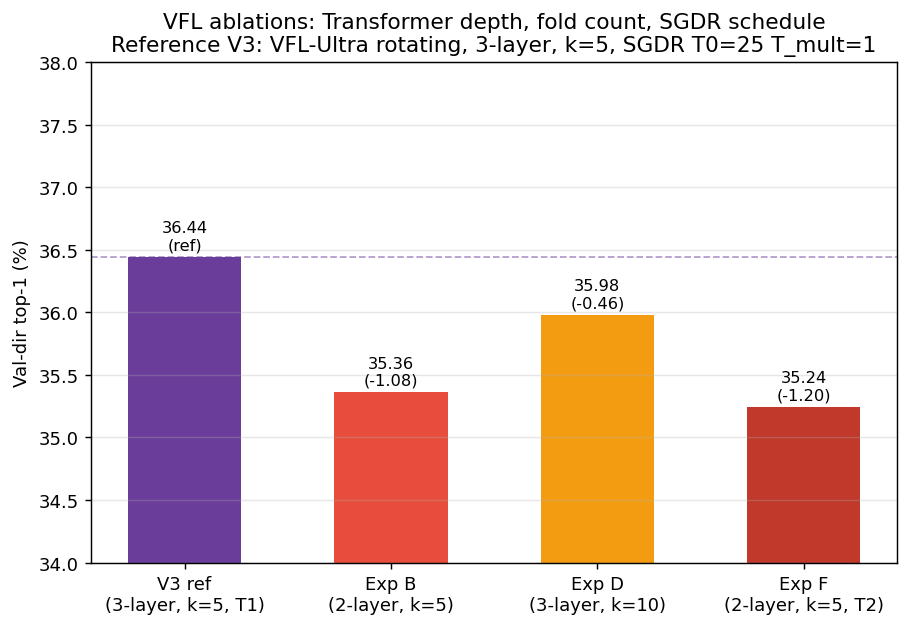
\includegraphics[width=\linewidth]{fig17_ablation_vfl.png}
  \caption{VFL ablations: Transformer depth (2 vs.\ 3 layers, $-1.08$\,pp for
  2 layers), fold count (5 vs.\ 10, $-0.46$\,pp for 10 folds --- VFL is
  data-saturated at $k{=}5$), and SGDR restart shape ($\leq 0.12$\,pp effect)
  (Sec.~\ref{sec:abl}).}
  \label{fig:abla_vfl}
\end{figure}

\begin{figure}[h]
  \centering
  
\includegraphics[width=\linewidth]{fig04_ensemble.png}
  \caption{Track~A ensemble vs.\ its components. Log-softmax late fusion of
  two TSM-ResNet18 variants, one VFL variant (all +TTA), the new
  TSM-ResNet50 and a CE-trained TSM ablation (no TTA) reaches $46.75\%$
  \texttt{val\_dir} and $0.4785$ public / $0.4547$ private on Kaggle ---
  our best closed-track submission (Sec.~\ref{sec:rotating}).}
  \label{fig:ensemble}
\end{figure}

\begin{figure}[h]
  \centering
  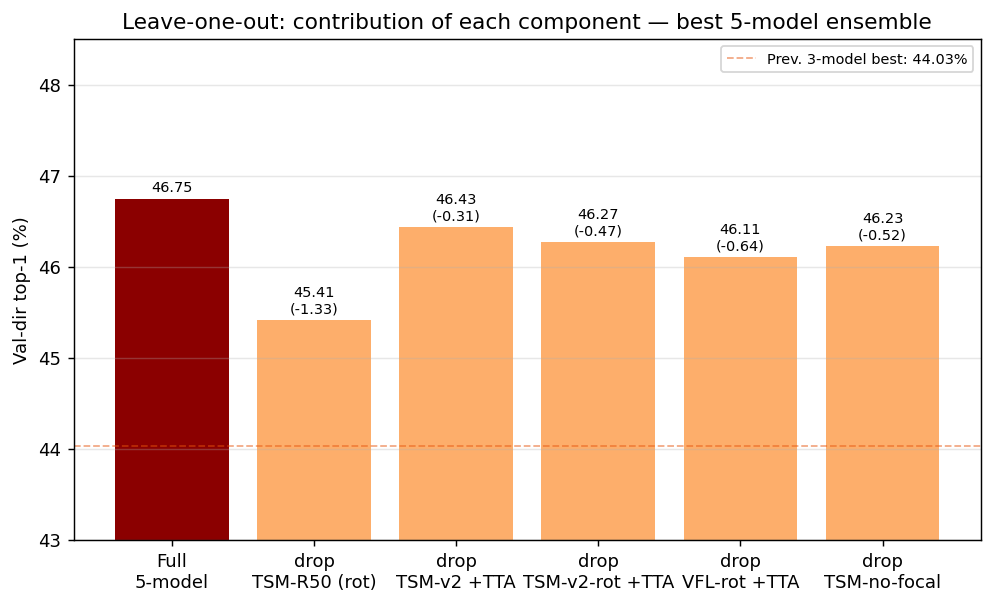
\includegraphics[width=\linewidth]{fig11_leave_one_out.png}
  \caption{Track~A leave-one-out study on the 5-model ensemble
  (\texttt{val\_dir} top-1). The ResNet50 backbone is the dominant
  contributor ($-1.33$\,pp), ahead of the architecturally distinct VFL
  ($-0.64$\,pp): backbone diversity outweighs family diversity here
  (Table~\ref{tab:loo}).}
  \label{fig:loo}
\end{figure}

\begin{figure}[h]
  \centering
  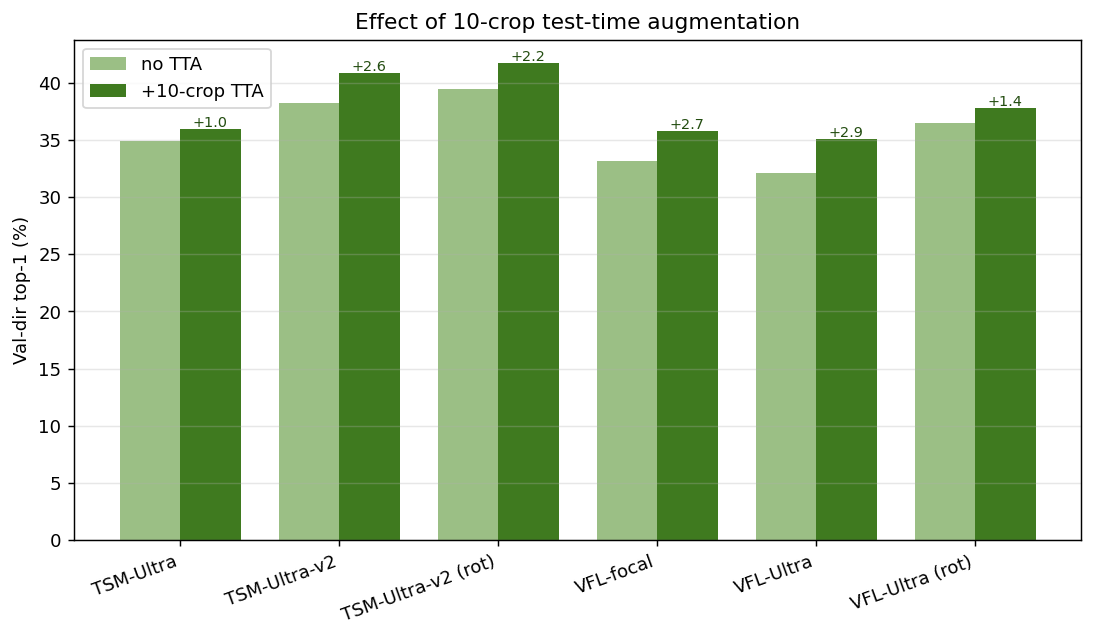
\includegraphics[width=\linewidth]{fig02_tta_effect.png}
  \caption{Effect of 10-crop spatial TTA on Track~A models. TTA adds
  ${\sim}1$\,pp on the strongest checkpoint and is essential at the ensemble
  level, where independent random errors from different crops average out
  (Sec.~\ref{sec:trackA}).}
  \label{fig:tta}
\end{figure}

\begin{figure}[h]
  \centering
  
\includegraphics[width=\linewidth]{fig12_tta_directional_tradeoff.png}
  \caption{TTA directional-class trade-off. Horizontal-flip TTA improves most
  classes but hurts a few direction-encoded ones
  (\emph{Pulling left$\rightarrow$right} vs.\ \emph{right$\rightarrow$left})
  even after the flip-aware logit remap, because mirror evidence is
  intrinsically ambiguous when motion is short.}
  \label{fig:ttatradeoff}
\end{figure}

\begin{figure}[h]
  \centering
  
\includegraphics[width=\linewidth]{fig03_rotating_effect.png}
  \caption{Rotating-fold training. Re-training the strongest checkpoints on
  every train/val fold yields snapshots that share weights but disagree on the
  boundary, contributing uncorrelated errors that the log-softmax ensemble
  exploits; the gain is larger for VFL ($+4.3$\,pp) than for TSM ($+1.2$\,pp)
  (Sec.~\ref{sec:rotating}).}
  \label{fig:rotating}
\end{figure}

\begin{figure}[h]
  \centering
  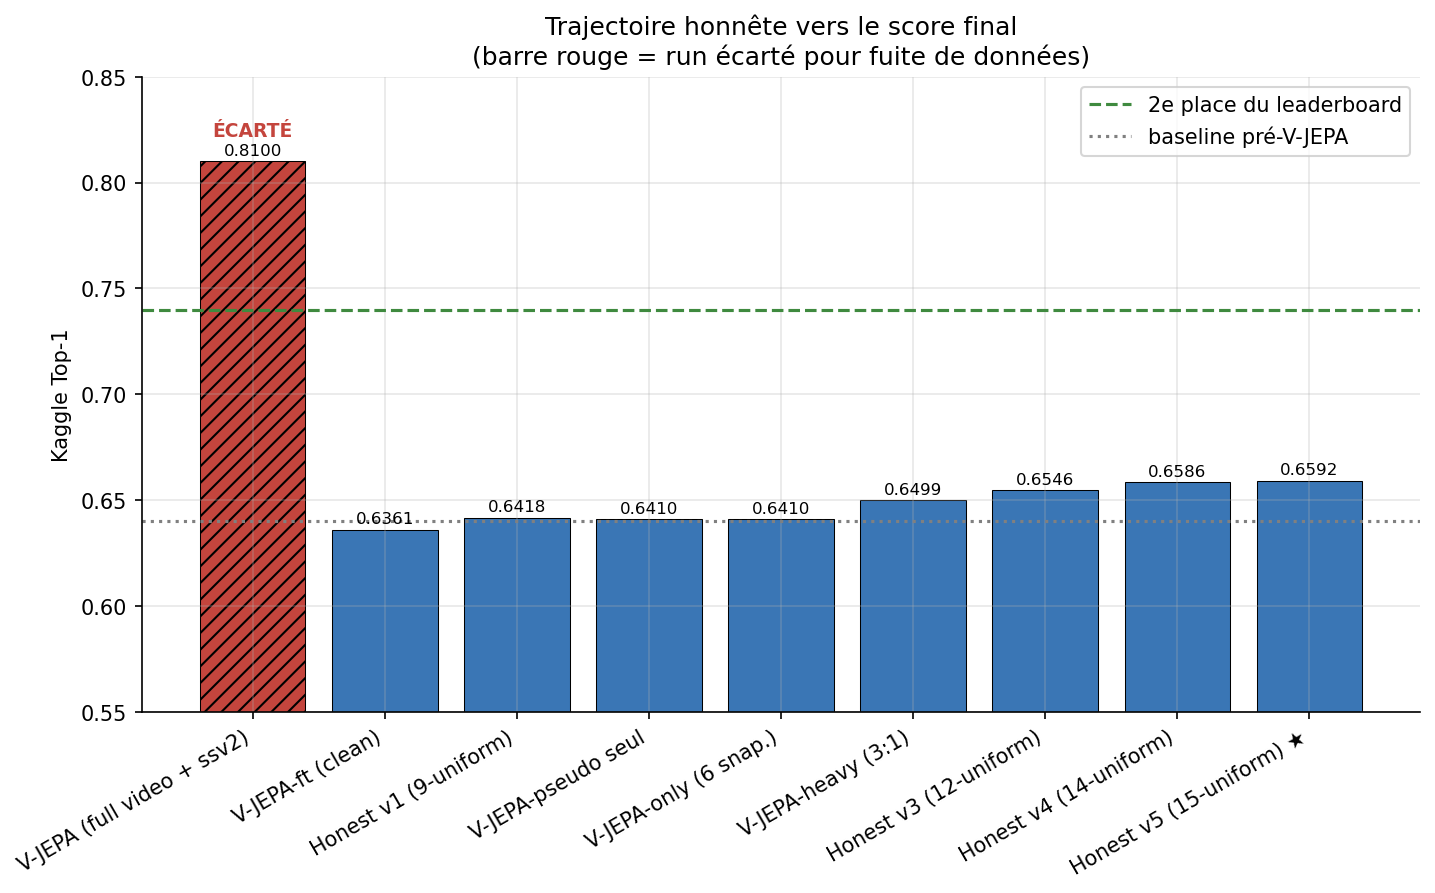
\includegraphics[width=\linewidth]{A_kaggle_journey.png}
  \caption{Track~B honest Kaggle progression. The discarded leaky submission
  ($0.81$, red) is plotted alongside every clean ensemble; each gain comes from
  adding architecturally distinct members, not from re-weighting. The dashed
  line marks the second-place public reference ($0.74$); the gap to it bounds
  what self-supervised pretraining + diverse ensembling buys us
  (Sec.~\ref{sec:results}, Table~\ref{tab:kaggle}).}
  \label{fig:kagglejourney}
\end{figure}

\begin{figure}[h]
  \centering
  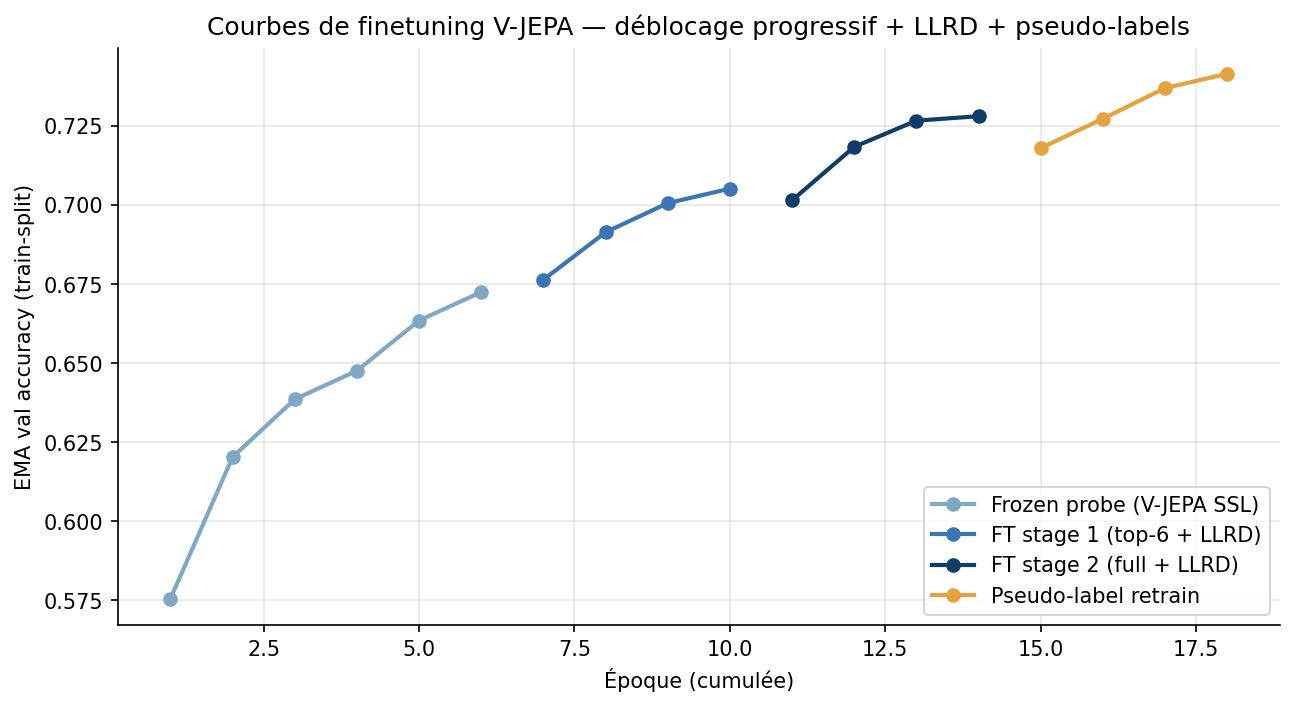
\includegraphics[width=\linewidth]{D_training_curves.png}
  \caption{V-JEPA progressive unfreezing + LLRD (Track~B internal val). Each
  phase warm-starts above the previous plateau: frozen probe ($0.55\!\to\!0.67$),
  then top-6 unfrozen + LLRD ($0.68\!\to\!0.71$), then full encoder
  ($0.70\!\to\!0.73$), then pseudo-label retrain ($0.72\!\to\!0.74$). The
  staircase pattern is the visual signature that LLRD has preserved each
  phase's feature geometry (Sec.~\ref{sec:trackB}).}
  \label{fig:vjepacurves}
\end{figure}

\begin{figure}[h]
  \centering
  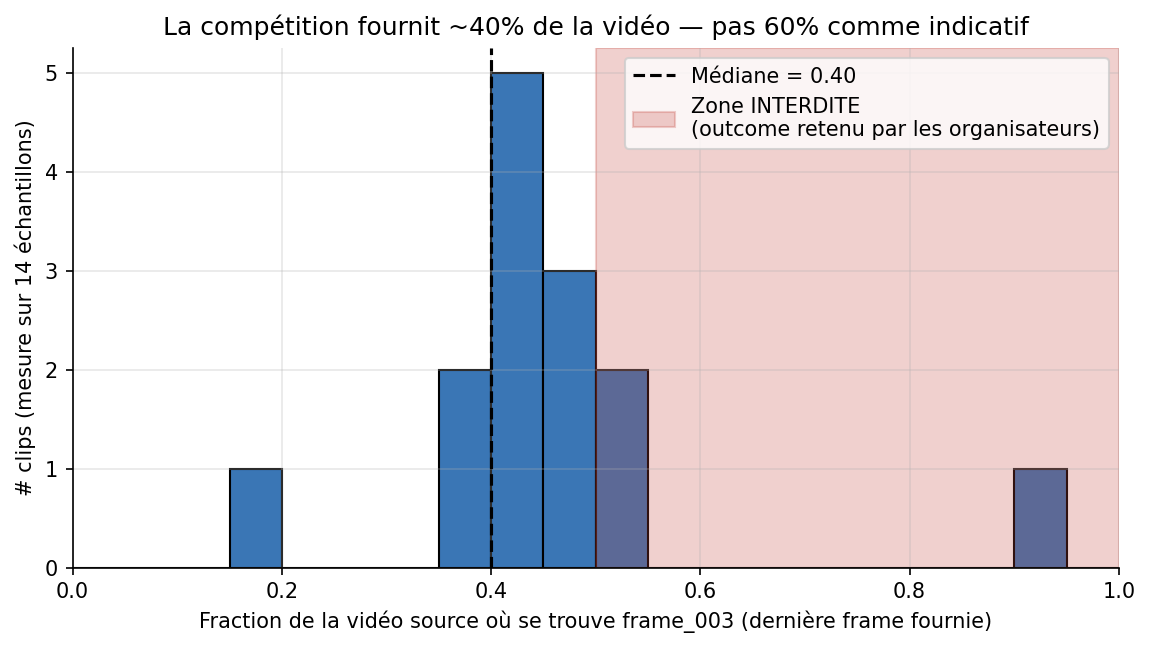
\includegraphics[width=\linewidth]{E_frame_position_histogram.png}
  \caption{Where shipped \texttt{frame\_003} sits in the source SSv2 clip
  (fraction). The dashed line at $0.40$ is the median end-of-window; the shaded
  region $[0.50,1.00]$ is the withheld outcome --- our re-extraction is
  hard-bounded to the un-shaded region (Sec.~\ref{sec:integrity}).}
  \label{fig:framehist}
\end{figure}

\begin{figure}[h]
  \centering
  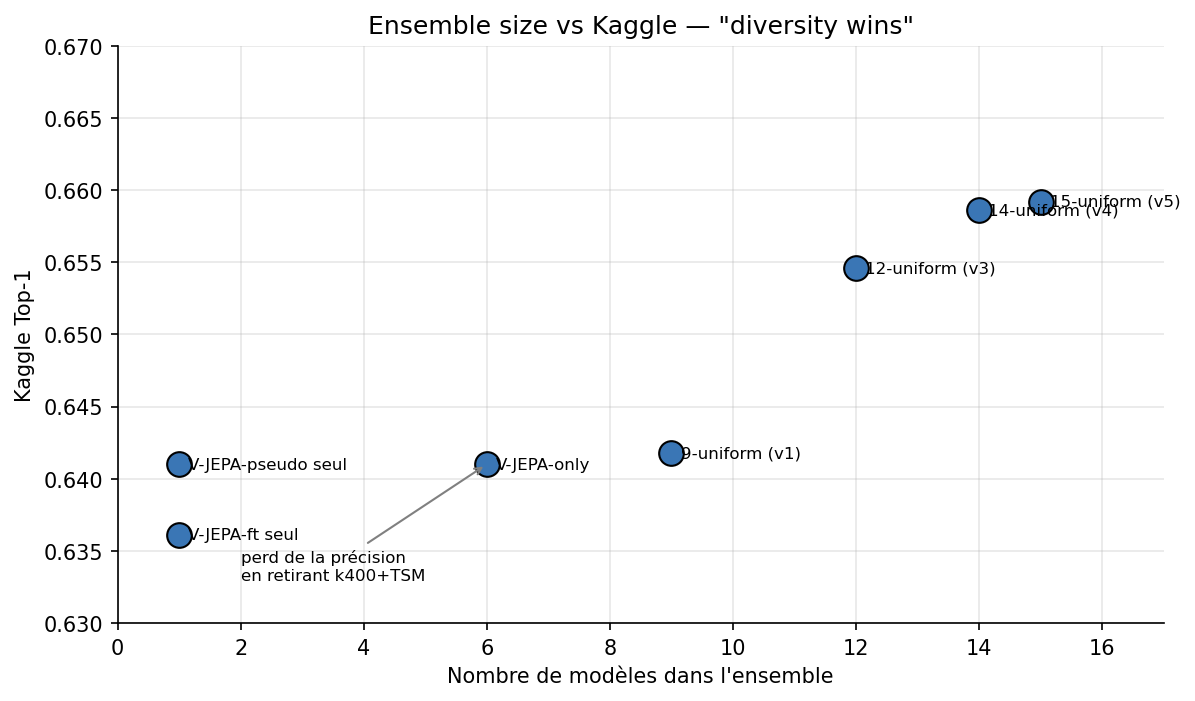
\includegraphics[width=\linewidth]{B_ensemble_size_vs_score.png}
  \caption{Track~B Kaggle vs.\ ensemble size. Returns from adding diverse
  honest members are still positive at $n{=}14$; at $n{=}6$, dropping K400
  + TSM \emph{hurts} despite their lower individual scores, because their
  uncorrelated errors disappear from the average
  (Table~\ref{tab:strategy}).}
  \label{fig:enssize}
\end{figure}

\begin{figure}[h]
  \centering
  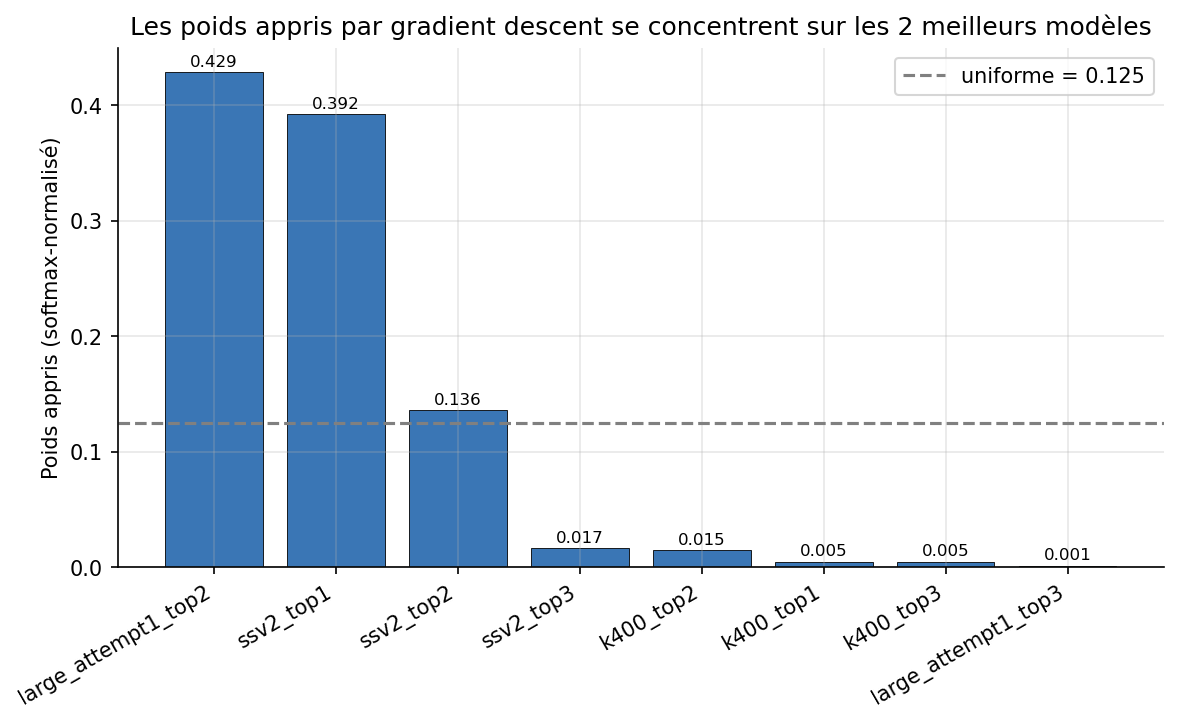
\includegraphics[width=\linewidth]{I_learned_weights_collapse.png}
  \caption{Learned ensemble weights collapse onto the two strongest members
  (${\sim}82\%$ of mass on \texttt{large\_attempt1\_top2} and
  \texttt{ssv2\_top1}), effectively zeroing K400 contributions. This is exactly
  why a learned weighting fails to beat uniform: it discards the very
  decorrelation signal that diverse weaker members provide
  (Sec.~\ref{sec:results}).}
  \label{fig:learnedw}
\end{figure}

\begin{figure*}[h]
  \centering
  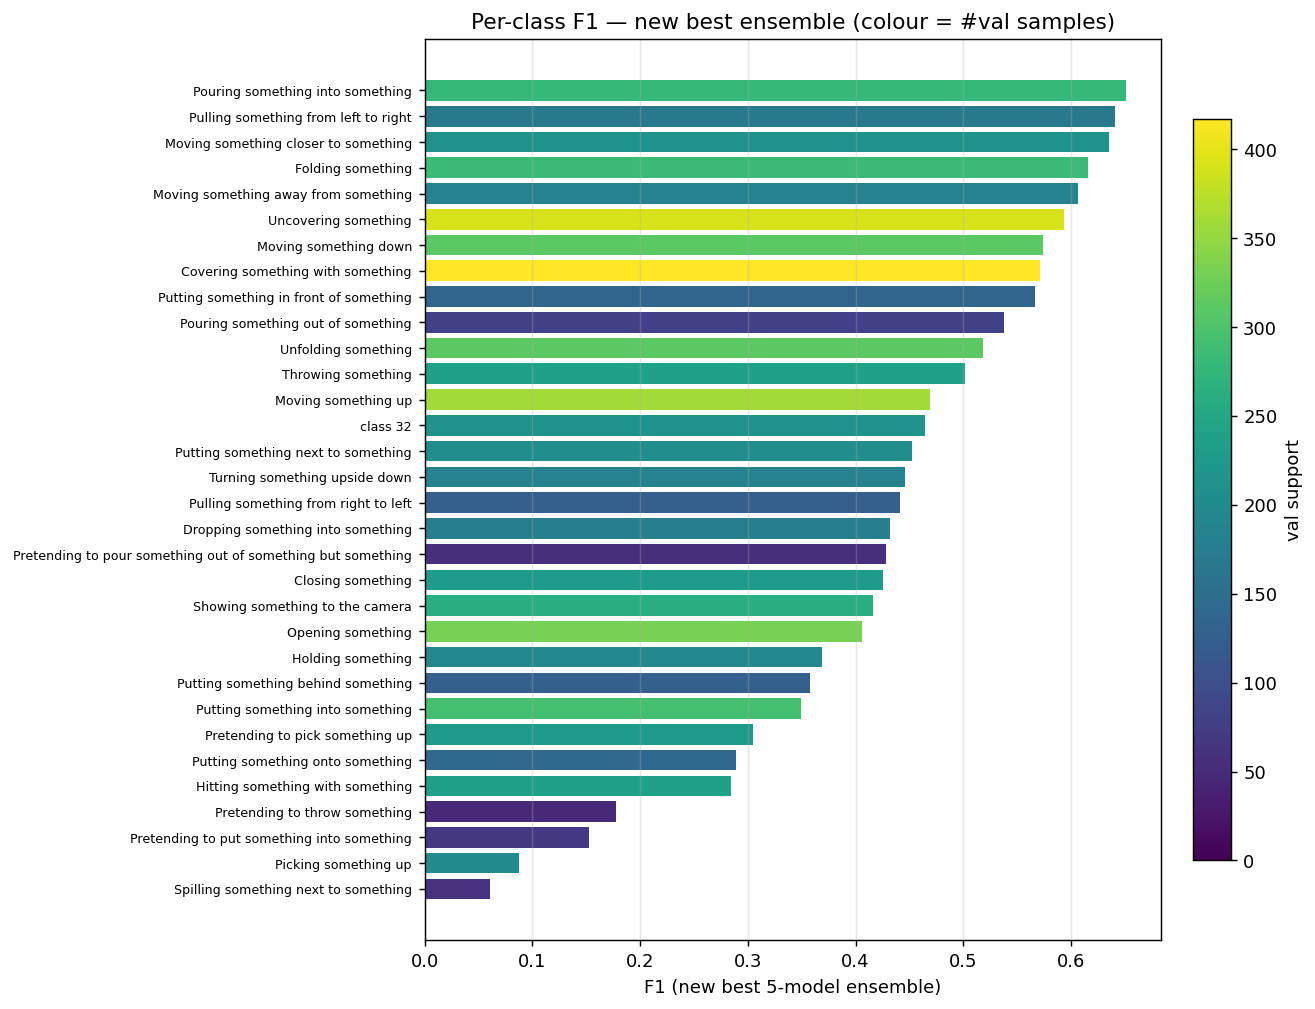
\includegraphics[width=0.95\textwidth]{fig05_per_class_f1.png}
  \caption{Per-class F1 (5-model ensemble, \texttt{val\_dir}). Directional
  single-object motions score highest; ``pretending'' and direction-ambiguous
  classes score lowest (Sec.~\ref{sec:failure}).}
  \label{fig:perclass}
\end{figure*}

\begin{figure*}[h]
  \centering
  
\includegraphics[width=0.95\textwidth]{fig06_confusion_matrix.png}
  \caption{$33\times33$ confusion matrix (5-model ensemble, \texttt{val\_dir}).
  Off-diagonal mass concentrates on semantically adjacent pairs (real vs.\
  pretended; fold vs.\ unfold; motion vs.\ \emph{holding}).}
  \label{fig:confmat}
\end{figure*}

\begin{figure*}[h]
  \centering
  
\includegraphics[width=0.95\textwidth]{fig07_confused_pairs.png}
  \caption{Most-confused class pairs. The dominant errors are intent (real vs.\
  pretended) and temporal-direction confusions (Sec.~\ref{sec:failure}).}
  \label{fig:pairs}
\end{figure*}

% =====================================================================
\clearpage
{\small
\bibliographystyle{ieeenat_fullname}
\bibliography{references}
}

\end{document}
